\documentclass[landscape,paperwidth=76.0in,paperheight=36.0in,fontscale=0.292]{baposter}

\usepackage[vlined]{algorithm2e}
\usepackage{times}
\usepackage{calc}
\usepackage{url}
\usepackage{graphicx}
\usepackage{amsmath}
\usepackage{amssymb}
\usepackage{relsize}
\usepackage{multirow}
\usepackage{booktabs}

\usepackage{graphicx}
\usepackage{multicol}
\usepackage[T1]{fontenc}
\usepackage{ae}
\usepackage{enumitem}

\usepackage{colortbl}
\usepackage{xcolor}
\usepackage{geometry}


\graphicspath{{images/}}

\setlist[itemize]{leftmargin=*,nosep}
 \setlength{\columnsep}{0.7em}
 \setlength{\columnseprule}{0mm}

 % Save space in lists. Use this after the opening of the list

 \newcommand{\compresslist}{%
 \setlength{\itemsep}{0pt}%
 \setlength{\parskip}{0pt}%
 \setlength{\parsep}{0pt}%
 }
\renewcommand{\rmdefault}{ptm} % Arial
\renewcommand{\sfdefault}{ptm} % Arial

\begin{document}
% Here starts the poster
\begin{poster}{
 % Show grid to help with alignment
 grid=false,
 columns=5,
 % Column spacing
 colspacing=0.7em,
 % Color style
 headerColorOne=cyan!20!white!90!black,
 borderColor=cyan!30!white!90!black,
 % Format of textbox
 textborder=bars,
 % Format of text header
 headerborder=open,
 headershape=roundedright,
 headershade=plain,
 background=none,
 bgColorOne=cyan!10!white,
 headerheight=0.12\textheight}
 % ========================================================
 % Eye Catcher
 {
      \includegraphics[width=0.05\linewidth]{ucCAL.png}
      \makebox[0.01\textwidth]{} 
      \raisebox{0.08\height}{\includegraphics[width=0.08\linewidth]{ancestry.jpg}}
      \makebox[0.04\textwidth]{} 
 }
 % Title
 {\sc\Huge\bf Ventral-Dorsal Neural Networks: Object Detection via Selective Attention}
 % Authors
 {\vspace{0.0em} Mohammad K. Ebrahimpour$^1$ , Jiayun Li$^2$, Yen-Yun Yu$^3$, Jackson L. Reese $^3$,  Azadeh Moghtaderi $^3$, Ming-Hsuan Yang$^1$, David C. Noelle$^1$  \\[0.2em]
  %{{\{mebrahimpour,mhyang,dnoelle\}@ucmerced.edu}, \texttt{\{jiayunli@\}@ucla.edu} , \texttt{\{yyu,jreese,amoghtaderi\}@ancestry.com}\\[0.2em] }
 {University of California, Merced $^1$, University of California, Los Angles$^2$, Ancestry.com $^3$\\[0.2em] }}
 % University logo
 {
    \begin{tabular}{r}
        \includegraphics[width=0.06\linewidth]{wacv.png}
    \end{tabular}
 }


% ========================================================
%                                               Inspirations                                                            
% ========================================================
\headerbox{\bf\color{blue} Brain Inspirations}{name=inspiration,column=0,row=0,span=2}{
    \textbf{\color{blue} Vision Streams:} Vision in the brain has two main streams called Ventral and Dorsal.
    \begin{center}
        \vspace{-0.8em}
        \centering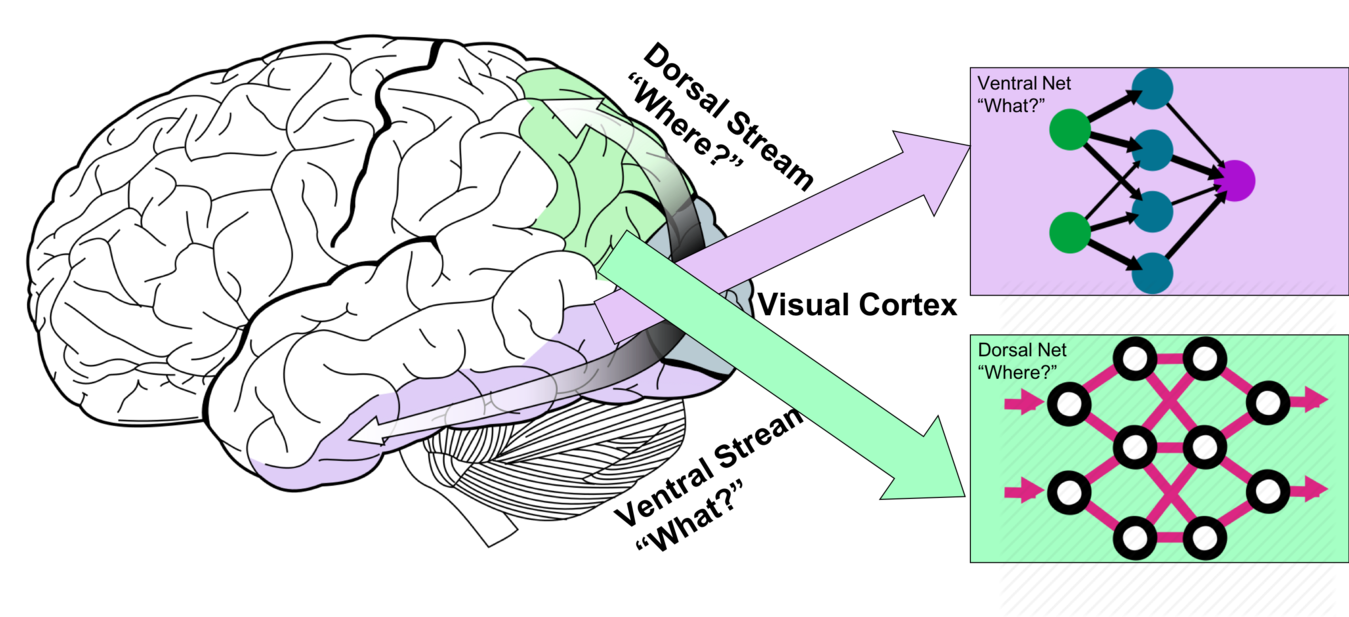
\includegraphics[width=0.6\linewidth]{images/brain0.png}
    \end{center}

    \vspace{-0.8em}
    \textbf{\color{blue}Brain Inspiration:}

    \begin{itemize}
        \item Ventral Pathway:  The ventral pathway from primary visual cortex, entering the temporal lobe, is dominated by ``what'' information.
        \item Dorsal Stream: The dorsal pathway, into the parietal lobe, is dominated by ``where'' information.
        \item Inspired by this structure, we propose the integration of
a ``Ventral Network'' and a ``Dorsal Network'', which are
complementary. Information about object identity can guide 
localization, and location information can guide attention to relevant
image regions, improving object recognition.
    \end{itemize}  
}

%========================================================
                                                 Literature Review
% ========================================================
\headerbox{\bf\color{blue} Literature Review}{name=LR,column=2,row=0,span=3}{
\begin{tabular}{cc}
\textbf{\color{blue} Region Proposal Based Framework} & \textbf{\color{blue} Single Shot Detectors} \\
\includegraphics[width=0.45\linewidth]{images/rcnn.png} &
\includegraphics[width=0.45\linewidth]{images/YOLO.jpg}\\

\end{tabular}    
}

% ========================================================
%                                                           Results
% ========================================================

% ------------------------------ Part 1 -----------------------------------------
\headerbox{\bf\color{blue} Experiments \& Results}{name=results,column=2,below=LR,span=3}{
    \begin{minipage}[t]{0.5\textwidth}
        \textbf{\color{blue}Object Detection Results:} 
        \vspace{-0.2em} 
        \begin{center}
           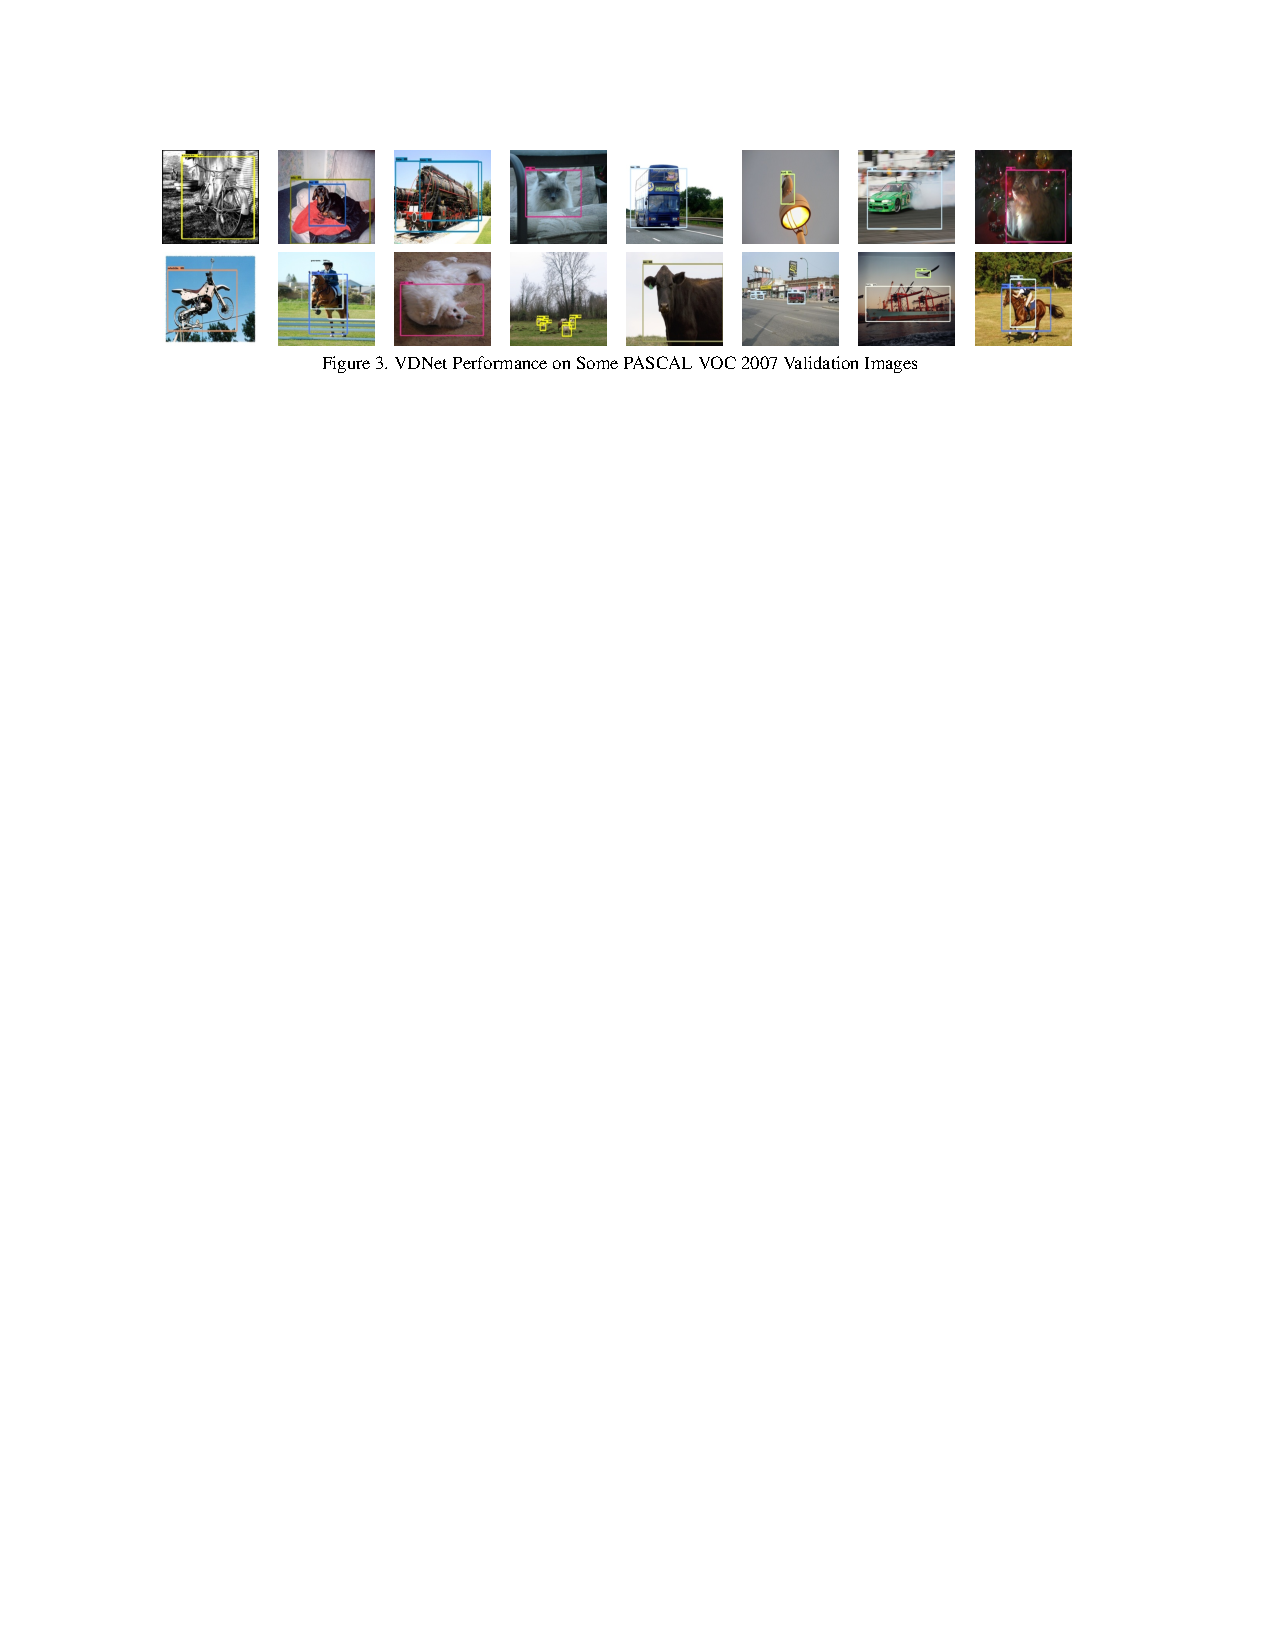
\includegraphics[width=\textwidth]{images/voc}
        \end{center}
    \end{minipage}
   \vspace{0.1em}
% ------------------------------ Part 2 ----------------------------------------
    \begin{minipage}[t]{0.5\textwidth}
        \textbf{\color{blue} mAP results on VOC 2007:}
        \vspace{-0.2em}
        \begin{center}
            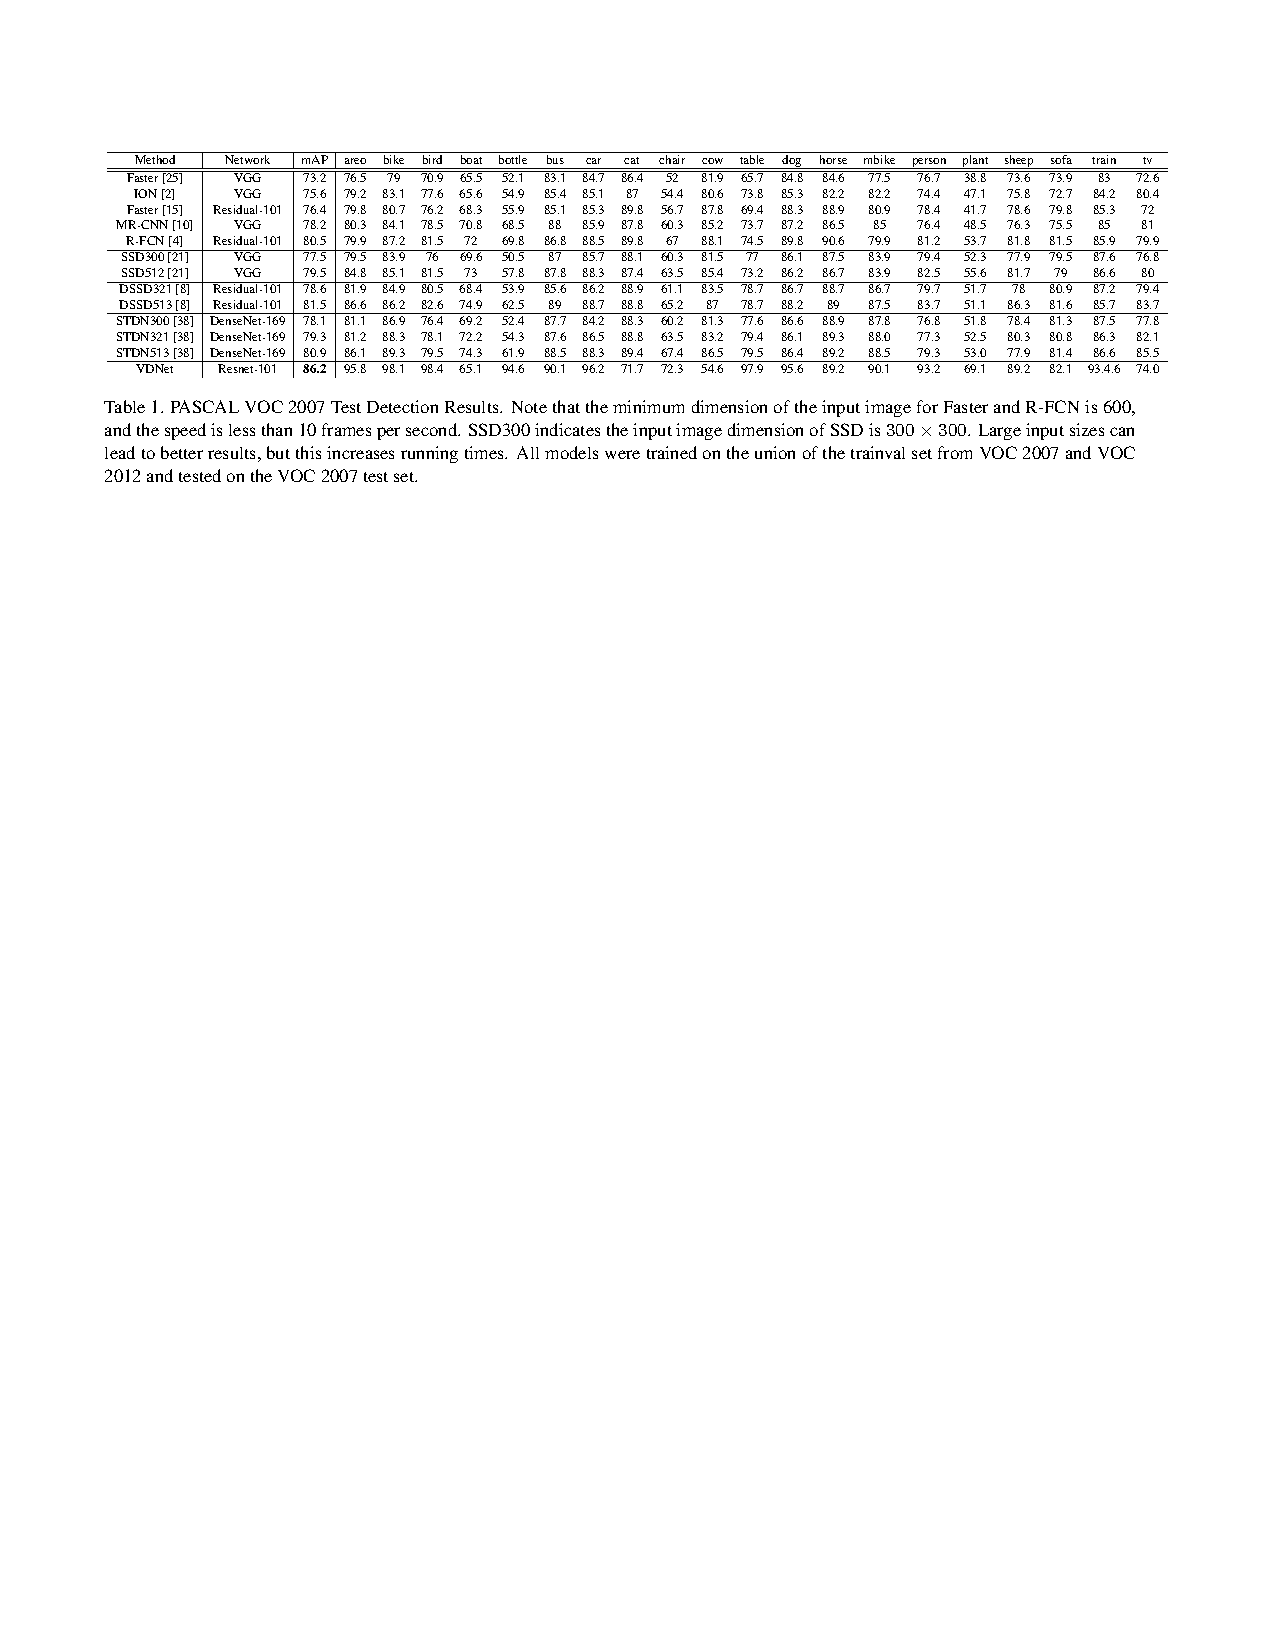
\includegraphics[width=\textwidth]{images/voc2007}
        \end{center}
        \vspace{-0.9em}
        \end{minipage}
    \hfill
% ------------------------------- Part 3 ---------------------------------------
    \begin{minipage}[t]{1.0\textwidth}
    \textbf{\color{blue}mAP results on VOC 2012:} 
        \begin{center}
            \vspace{-0.2em}
            \includegraphics[width=\textwidth]{images/voc2012}
        \end{center}
    \end{minipage}

    \vspace{0.1em}

% -------------------------------- Part 4 --------------------------------------

 \begin{minipage}[t]{0.33\textwidth}
        \textbf{\color{blue}Object Detection Results:} 
        \vspace{-1.0em}
   
        \begin{center}
           \includegraphics[width=1.0\textwidth]{images/depth}
        \end{center}
    \end{minipage}
    \begin{minipage}[t]{0.33\textwidth}
        \textbf{\color{blue} Selective Attention:} 
        \vspace{-0.8em}
        \begin{center}
            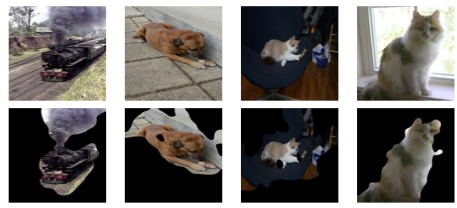
\includegraphics[width=0.82\textwidth]{images/sa}
        \end{center}
   \end{minipage}
       \begin{minipage}[t]{0.34\textwidth}
        \textbf{\color{blue} Ventral -Dorsal Networks on Github:} 
     %  \vspace{-1.0em}
        \begin{center}
            \includegraphics[width=0.35\textwidth]{images/VDNet_QR.png}
       \end{center}
   \end{minipage}
}
%=========================================================







% ========================================================
\headerbox{\bf\color{blue} Dual Networks: Ventral and Dorsal}{name=formulation,column=0,below=inspiration,span=2}{
    \vspace{-0.5em}
    \begin{center}
     \includegraphics[width=0.9\textwidth]{images/VDNet_copy.png}
    \end{center}
   \vspace{-0.5em}

  %  \vspace{-0.5em} 
\textbf{Gestalt Total (GT):}\\
For a given image, let $f(x,y,k)$ denote the activation of the last convolutional layer at spatial location $(x,y)$. The ``Gestalt Total" activation is defined as:
\vspace{-3mm}
\begin{equation}
\label{e:CAM}
GT = \sum_{k}\sum_{x,y} f(x,y,k)
\end{equation}
\textbf{Sensitivity Analysis:}\\
\begin{equation}
S = \left. {\frac{\partial \ GT}{\partial \ X}}\ \right|_{X=I}
\label{eq:sensitivity}
\end{equation}
where $I$ denotes the current image.\\
\textbf{Loss Function:}\\
\begin{equation}
\begin{split}
L(p_i,t_i) = \frac{1}{N_{cls}}\sum_i L_{cls}(p_i,p_i^{\ast}) 
+\lambda \frac{1}{N_{reg}} \sum_i p_i^{\ast} L_{reg}(t_i,t_i^{\ast}).
\end{split}
\label{eq:objFunction}
\end{equation}
\vspace{10cm}
}

%%%%%%%%%%%%%%%%%%%%%%%%%%%%%%%%%%%%%%%%%%%%%%%%%%%%%%%%%%%%%%%%%%%%%%%%%%%%%%
%\headerbox{\bf\color{blue} Dual Networks: Ventral and Dorsal}{name=abstract,column=0,below=formulation,span=2}{
 %   \textbf{\color{blue}Network Architecture:} PS-FCN consists of three components, namely a shared-weight feature extractor, a fusion layer, and a normal regression network.
%    \vspace{-0.5em}
%    \begin{center}
%     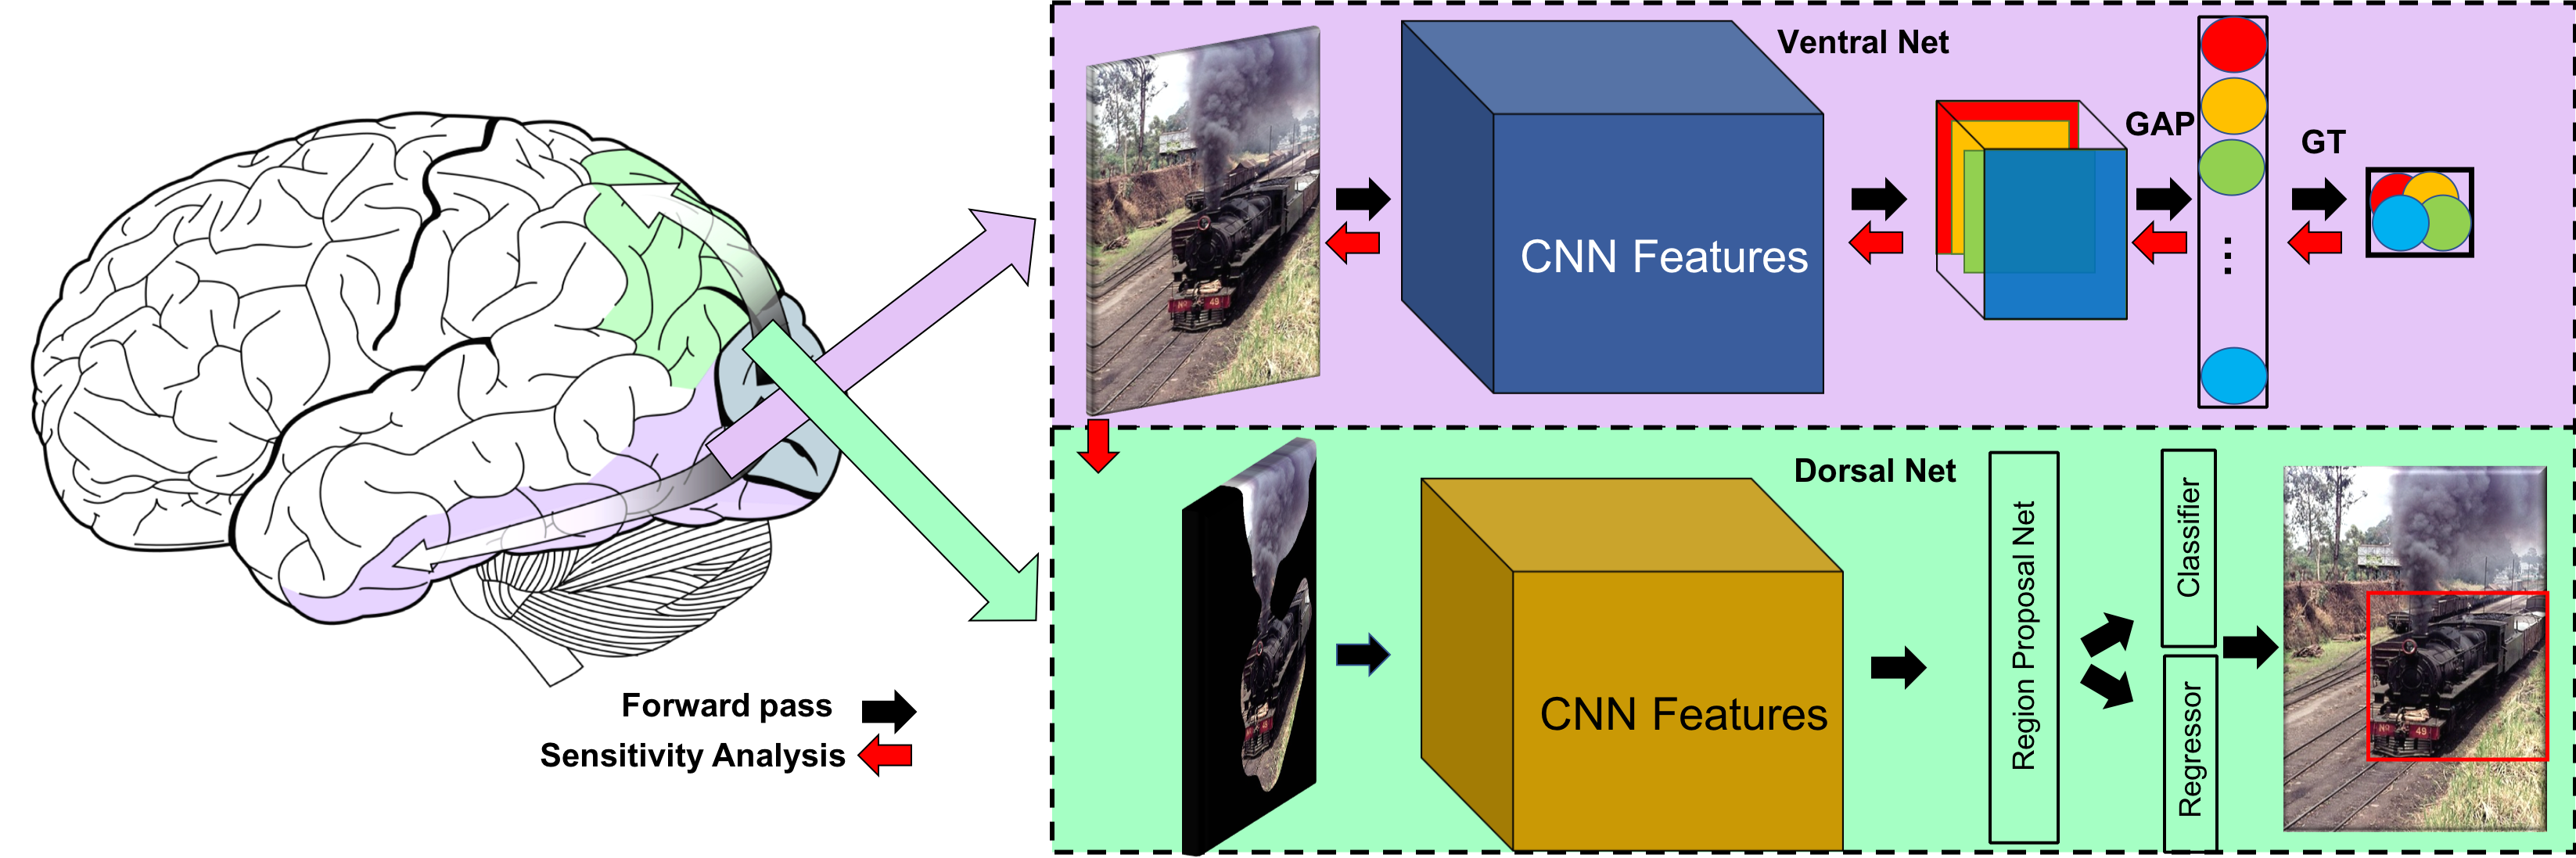
\includegraphics[width=0.7\textwidth]{images/VDNet.png}
%    \end{center}
%    \vspace{-0.5em}
%    \textbf{\color{blue}Loss function:}
 %   \vspace{-0.5em} 

%}
%\vspace{-3mm}
\end{poster}
\end{document}
